%% Beispiel-Präsentation mit LaTeX Beamer im KIT-Design
%% entsprechend den Gestaltungsrichtlinien vom 1. August 2020
%%
%% Siehe https://sdqweb.ipd.kit.edu/wiki/Dokumentvorlagen

%% Beispiel-Präsentation
\documentclass[en]{sdqbeamer} 
 
%% Titelbild
\titleimage{banner_2020_kit}

%% Gruppenlogo
\grouplogo{CEL_logo.png}

%% Gruppenname und Breite (Standard: 50 mm)
\groupname{Communications Engineering Lab (CEL)\hspace{3mm}\raisebox{-.43\height}{
\includegraphics[height=7 mm]{logos/CEL_logo.png}}}
\groupnamewidth{90mm}

% Beginn der Präsentation

\title[Research internship]{Direct Detection with Phase Recovery in Optical Communications}
\subtitle{Research internship from 5.\,2023 to 11.\,2023} 
\author[Diego Figueroa]{Diego Alejandro Figueroa Del Castillo }

\date[16.\,1.\,2024]{16. January 2024}

% Literatur 
 
\usepackage[citestyle=authoryear,bibstyle=numeric,hyperref,backend=biber]{biblatex}
\addbibresource{presentation.bib}
\bibhang1em


\usepackage{graphics,bm}
\setbeamercovered{transparent}
\usepackage{tikz}
\usetikzlibrary{positioning} 
\usetikzlibrary{matrix}
\usepackage{siunitx}
\usepackage{slashbox}

\usefonttheme[onlymath]{serif}

\usepackage{pgfplots}
\usepgfplotslibrary{groupplots}
\pgfplotsset{compat=1.17}
\pgfdeclarelayer{background layer}%
\pgfdeclarelayer{foreground layer}%
\pgfsetlayers{background layer,main,foreground layer}%
\usepackage{subcaption}
\usepackage{upgreek}
\usepackage{dsfont}
\setbeamertemplate{caption}[numbered]

\DeclareMathOperator*{\argmax}{arg\,max}

\tikzset{
  invisible/.style={opacity=0},
  visible on/.style={alt={#1{}{invisible}}},
  alt/.code args={<#1>#2#3}{%
    \alt<#1>{\pgfkeysalso{#2}}{\pgfkeysalso{#3}} % \pgfkeysalso doesn't change the path
  },
}



%%%%%%%%%%%%%%%%%%%%%%%%%%%%%%%%%%%%%
\begin{document}
 
%Titelseite
\KITtitleframe

%Inhaltsverzeichnis
\begin{frame}[allowframebreaks]{Table of contents}
\tableofcontents[sections={1-2}]
    \framebreak
  \tableofcontents[sections={3-4}]
\end{frame}



\section{Introduction}

\begin{frame}{}{}
\center\Huge Introduction
\end{frame}

\subsection{Motivation}

\begin{frame}{Motivation}{}
Square-law detection, also known as Direct detection (DD), is a detection scheme that measures the square magnitude of a complex waveform.
\begin{itemize}
\item Nonlinear detection
\item Used specifically in short-haul systems (up to \SI{50}{\km})
\end{itemize}

\begin{greenblock}{Why is Direct Detection relevant?}
	\begin{itemize}
\item The receiver hardware is simple
\item Low-cost alternative compared to the coherent detection
\end{itemize}
\end{greenblock}
\end{frame}


\subsection{Direct detection}
\begin{frame}{Direct detection}{}
Direct Detection is performed with a single photodiode that converts the optical signal into an electric signal. 
\begin{align}
I_p&=R_d\cdot P_\text{in}\\
 P_\text{in}&\propto E_\text{in}^2
\end{align}

The detection is affected by the shot and thermal noise.
\begin{align}
I(t) = I_p+i_s(t)+i_{th}(t)
\end{align}
with $i_s(t)\sim\mathcal{N}(0,\sigma_s^2)$ and $i_{th}(t)\sim\mathcal{N}(0,\sigma_{th}^2)$, and 
\begin{align}
\sigma_s^2 &= 2qI_pB &&\sigma_{th}^2 = \frac{4k_BT}{R_L} F_nB
\end{align}
\end{frame}


\subsection{Capacity under direct detection}
\begin{frame}{Capacity under direct detection}{}
Direct Detection can retrieve only the information about the magnitude of the signal, so it is reasonable to think that the capacity of this system should be reduced by a half.
\begin{greenblock}{Capacity loss}
In \cite{Mecozzi_2018,Tasbihi_Capacity} it is shown that the spectra efficiency of a band-limited or time-limited system under Direct Detection  is at most \SI{1}{bit/\s/\Hz} less than the same system under coherent detection.
\begin{align}
	I_\text{CD}-1\leq I_\text{DD}\leq I_\text{CD}
\end{align}

\end{greenblock}

\end{frame}



\subsection{Basic principle of phase recovery}
\begin{frame}{Basic principle of phase recovery}{}
Given two complex numbers $z_1$ and $z_2$; from $|z_1|^2$, $|z_2|^2$ and $|z_1+z_2|^2$ (an ISI term), it is possible to determine the phase difference between $z_1$ and $z_2$ up to a sign ambiguity.
\begin{align*}
	|z_1+z_2|^2 &= (z_1+z_2)(z_1+z_2)^* \\
	&=z_1z_1^*+z_1z_2^*+z_2z_2^*+z_1^*z_2\\
	&=|z_1|^2+|z_2|^2+z_1z_2^*+\bigl(z_1z_2^*\bigr)^*\\
	&=|z_1|^2+|z_2|^2+2\text{Re}\{z_1z_2^*\}\\
\end{align*}%
under the convention that $z_1 = a\cdot e^{j\alpha}$ and $z_2 = b\cdot e^{j\beta}$%
\begin{equation}
	|z_1+z_2|^2 =|z_1|^2+|z_2|^2+2|z_1||z_2|\cos(\alpha-\beta)
	\label{eq:square_mag_of_sum}
\end{equation}

\end{frame}


\begin{frame}{Basic principle of phase recovery}{}


\begin{columns}
	\column{.5\textwidth}
	\begin{figure}
\begin{center}

\begin{tikzpicture}
\begin{groupplot}[
group style={
    group name=my plots,
    group size=1 by 2,  % 1 row and 2 columns
    horizontal sep=1.5cm,  % Adjust horizontal separation between subplots
    vertical sep=-0.3cm,  % Adjust horizontal separation between subplots
  },
  width = 6cm,
  height = 4cm,
  xlabel={$t/T_s$},
  axis x line=middle,  % Show only the x-axis
  axis y line=none,    % Hide the y-axis
  xmin=-1.5, xmax=2.5,
  ymin=-0.6, ymax=0.6,  % Set ymax to 2
  xtick={-2,-1.5,...,2},
  xticklabels={-2,,-1,,0,,1,,2},
  tick label style={font=\scriptsize},
  xlabel style={
    right,
  },
]

\nextgroupplot
\begin{pgfonlayer}{background layer}
\addplot[kit-green100, domain=-1:1, samples=100, draw=none, fill=kit-green100, fill opacity=0.25] {0.25*(1+cos(deg(pi*x)))};
\addplot[kit-green100, domain=0:2, samples=100, draw=none, fill=kit-green100, fill opacity=0.25] {0.25*(1+cos(deg(pi*(x-1))))};
\end{pgfonlayer}
\addplot[kit-green100, domain=-1:1, samples=100, dashed, thick ] {0.25*(1+cos(deg(pi*x)))};
\addplot[kit-green100, domain=0:2, samples=100, dashed, thick] {0.25*(1+cos(deg(pi*(x-1))))};

\addplot[kit-red100, domain=-1:0, samples=100, thick] {0.25*(1+cos(deg(pi*x)))};
\addplot[kit-red100, domain=0:1, samples=100, thick] {0.25*(1+cos(deg(pi*x)))+0.25*(1+cos(deg(pi*(x-1))))};
\addplot[kit-red100, domain=1:2, samples=100, thick] {0.25*(1+cos(deg(pi*(x-1))))};
\addplot[only marks, mark=*, mark size=1.5pt, mark options={draw=kit-red100, fill=kit-red100!20}] coordinates{(0,0.5)(1, 0.5)};

\coordinate (p1) at (axis cs: 0,0.35);
\coordinate (p2) at (axis cs: 1,0.35);
\coordinate (top11) at (axis cs:0,\pgfkeysvalueof{/pgfplots/ymax});
\coordinate (top12) at (axis cs:0.5,\pgfkeysvalueof{/pgfplots/ymax});
\coordinate (top13) at (axis cs:1,\pgfkeysvalueof{/pgfplots/ymax});

\nextgroupplot
\begin{pgfonlayer}{background layer}
\addplot[kit-green100, domain=-1:1, samples=100, draw=none, fill=kit-green100, fill opacity=0.25] {0.25*(1+cos(deg(pi*x)))};
\addplot[kit-green100, domain=0:2, samples=100, draw=none, fill=kit-green100, fill opacity=0.25] {-0.25*(1+cos(deg(pi*(x-1))))};
\end{pgfonlayer}
\addplot[kit-green100, domain=-1:1, samples=100, dashed, thick ] {0.25*(1+cos(deg(pi*x)))};
\addplot[kit-green100, domain=0:2, samples=100, dashed, thick] {-0.25*(1+cos(deg(pi*(x-1))))};


\addplot[kit-red100, domain=-1:0, samples=100, thick] {0.25*(1+cos(deg(pi*x)))};
\addplot[kit-red100, domain=0:1, samples=100, thick] {0.25*(1+cos(deg(pi*x)))-0.25*(1+cos(deg(pi*(x-1))))};
\addplot[kit-red100, domain=1:2, samples=100, thick] {-0.25*(1+cos(deg(pi*(x-1))))};
\addplot[only marks, mark=*, mark size=1.5pt, mark options={draw=kit-red100, fill=kit-red100!20}] coordinates{(0,0.5)(1,- 0.5)};

\coordinate (p5) at (axis cs: 0,0.35);
\coordinate (p6) at (axis cs: 1,-0.35);
\coordinate (bot11) at (axis cs:0,\pgfkeysvalueof{/pgfplots/ymin});
\coordinate (bot12) at (axis cs:0.5,\pgfkeysvalueof{/pgfplots/ymin});
\coordinate (bot13) at (axis cs:1,\pgfkeysvalueof{/pgfplots/ymin});

\end{groupplot}

\begin{pgfonlayer}{background layer}
\draw [thick, dotted,-stealth, black!50] (top11) -- (bot11) --+ (0,-0.2) node [below, black, font=\scriptsize] {$y_0$};
\draw [thick, dotted,-stealth, black!50] (top13) -- (bot13) --+ (0,-0.2) node [below, black, font=\scriptsize] {$y_1$};
\end{pgfonlayer}

\node  at (p1) [font=\scriptsize, text=kit-green100]{$+1$};
\node  at (p2) [font=\scriptsize, text=kit-green100]{$+1$};
\node  at (p5) [font=\scriptsize, text=kit-green100]{$+1$};
\node  at (p6) [font=\scriptsize, text=kit-green100]{$-1$};



\end{tikzpicture}


\caption{Coherent Detection}
\label{default}
\end{center}
\end{figure}

	
	\column{.5\textwidth}
	\begin{figure}
\begin{center}

\begin{tikzpicture}
\begin{groupplot}[
group style={
    group name=my plots,
    group size= 1 by 2,  % 1 row and 2 columns
    horizontal sep=1.5cm,  % Adjust horizontal separation between subplots
    vertical sep=-0.3cm,  % Adjust horizontal separation between subplots
  },
  width = 6cm,
  height = 4cm,
  xlabel={$t/T_s$},
  axis x line=middle,  % Show only the x-axis
  axis y line=none,    % Hide the y-axis
  xmin=-1.5, xmax=2.5,
  ymin=-0.6, ymax=0.6,  % Set ymax to 2
  xtick={-2,-1.5,...,2},
  xticklabels={-2,,-1,,0,,1,,2},
  tick label style={font=\scriptsize},
  xlabel style={
    right,
  },
]%

\nextgroupplot
\begin{pgfonlayer}{background layer}
\addplot[kit-green100, domain=-1:1, samples=100, draw=none, fill=kit-green100, fill opacity=0.25] {0.25*(1+cos(deg(pi*x)))};
\addplot[kit-green100, domain=0:2, samples=100, draw=none, fill=kit-green100, fill opacity=0.25] {0.25*(1+cos(deg(pi*(x-1))))};
\end{pgfonlayer}

\addplot[kit-green100, domain=-1:1, samples=100, dashed, thick] {0.25*(1+cos(deg(pi*x)))};
\addplot[kit-green100, domain=0:2, samples=100, dashed, thick] {0.25*(1+cos(deg(pi*(x-1))))};


\addplot[kit-blue100, domain=-1:0, samples=100, thick] {2*(0.25*(1+cos(deg(pi*x))))^2};
\addplot[kit-blue100, domain=0:1, samples=100, thick] {2*(0.25*(1+cos(deg(pi*x)))+0.25*(1+cos(deg(pi*(x-1)))))^2};
\addplot[kit-blue100, domain=1:2, samples=100, thick] {2*(0.25*(1+cos(deg(pi*(x-1)))))^2};
\addplot[only marks, mark=*, mark size=1.5pt, mark options={draw=kit-blue100, fill=kit-blue100!20}] coordinates{(0,0.5)(1, 0.5)};
\addplot[only marks, mark=square*, mark size=1.5pt, mark options={draw=kit-blue100, fill=kit-blue100!20}] coordinates{(0.5, 0.5)};

\coordinate (p3) at (axis cs: 0,0.35);
\coordinate (p4) at (axis cs: 1,0.35);
\coordinate (top21) at (axis cs:0,\pgfkeysvalueof{/pgfplots/ymax});
\coordinate (top22) at (axis cs:0.5,\pgfkeysvalueof{/pgfplots/ymax});
\coordinate (top23) at (axis cs:1,\pgfkeysvalueof{/pgfplots/ymax});

\nextgroupplot
\begin{pgfonlayer}{background layer}
\addplot[kit-green100, domain=-1:1, samples=100, dashed, thick, fill=kit-green100, fill opacity=0.25] {0.25*(1+cos(deg(pi*x)))};
\addplot[kit-green100, domain=0:2, samples=100, dashed, thick, fill=kit-green100, fill opacity=0.25] {-0.25*(1+cos(deg(pi*(x-1))))};
\end{pgfonlayer}

\addplot[kit-blue100, domain=-1:0, samples=100, thick] {2*(0.25*(1+cos(deg(pi*x))))^2};
\addplot[kit-blue100, domain=0:1, samples=100, thick] {2*(0.25*(1+cos(deg(pi*x)))-0.25*(1+cos(deg(pi*(x-1)))))^2};
\addplot[kit-blue100, domain=1:2, samples=100, thick] {2*(0.25*(1+cos(deg(pi*(x-1)))))^2};
\addplot[only marks, mark=*, mark size=1.5pt, mark options={draw=kit-blue100, fill=kit-blue100!20}] coordinates{(0,0.5)(1, 0.5)};
\addplot[only marks, mark=square*, mark size=1.5pt, mark options={draw=kit-blue100, fill=kit-blue100!20}] coordinates{(0.5, 0)};

\coordinate (p7) at (axis cs: 0,0.35);
\coordinate (p8) at (axis cs: 1,-0.35);
\coordinate (bot21) at (axis cs:0,\pgfkeysvalueof{/pgfplots/ymin});
\coordinate (bot22) at (axis cs:0.5,\pgfkeysvalueof{/pgfplots/ymin});
\coordinate (bot23) at (axis cs:1,\pgfkeysvalueof{/pgfplots/ymin});


\end{groupplot}

\begin{pgfonlayer}{background layer}
\draw [thick, dotted,-stealth, black!50] (top21) -- (bot21) --+ (0,-0.2) node [below, black, font=\scriptsize] {$y_0$};
\draw [thick, dotted,-stealth, black!50] (top22) -- (bot22) --+ (0,-0.2) node [below, black, font=\scriptsize] {$y_1$};
\draw [thick, dotted,-stealth, black!50] (top23) -- (bot23) --+ (0,-0.2) node [below, black, font=\scriptsize] {$y_2$};
\end{pgfonlayer}

\node  at (p3) [font=\scriptsize, text=kit-green100]{$+1$};
\node  at (p4) [font=\scriptsize, text=kit-green100]{$+1$};
\node  at (p7) [font=\scriptsize, text=kit-green100]{$+1$};
\node  at (p8) [font=\scriptsize, text=kit-green100]{$-1$};


\end{tikzpicture}


\caption{Direct detection}
\label{default}
\end{center}
\end{figure}

	
\end{columns}


\end{frame}
%
%
%%%%%%%%%%%%%%%%%%%%%%%%%%%%%%%%%%%%%%
\section{Tukey signaling}
\begin{frame}{}{}
\center\Huge Tukey signaling
\end{frame}


\subsection{System model}

\begin{frame}{System model}{}

\begin{figure}
\begin{center}
\scalebox{1}{%
\begin{tikzpicture}[>=stealth,thick]%
\node [rectangle, draw, text width = 3cm, align = center, rotate=90,anchor=north] (CR) at (0,0) {Class\\Representative};
\node [rectangle, draw, text width = 3cm, align = center, rotate=90,anchor=north] (Sig) at($(CR.south)+(1,0)$) {Signaling};
\node [rectangle, draw, text width = 3cm, align = center, rotate=90,anchor=north] (DP) at($(Sig.south)+(1,0)$) {Dispersion\\Precompensation};
\node [circle, minimum width = 0.5cm, draw, rotate=90,anchor=north] (circ1) at($(DP.south)+(1,0)$) {};
\node [circle, minimum width = 0.5cm, draw, rotate=90,anchor=north] (circ2) at($(DP.south)+(1.3,0)$) {};
\node [rectangle, draw, text width = 3cm, align = center, rotate=90,anchor=north] (PD) at($(circ2.south)+(1,0)$) {Photodiode};
\node [rectangle, draw, text width = 3cm, align = center, rotate=90,anchor=north] (ID) at($(PD.south)+(1,0)$) {Integrate\\and Dump};
\node [rectangle, draw, text width = 3cm, align = center, rotate=90,anchor=north] (Det) at($(ID.south)+(1,0)$) {Detector};

\draw [->] (-1,0) -- node [above] {$k$}(CR); 
\draw [->] (CR.south) -- node [above] {$\bm x_k$} (Sig); 
\draw [->] (Sig.south) --  node [above] {$x(t)$} (DP); 
\draw [->] (DP.south) --  node [above] {$u(t)$} (circ1); 
\draw [->] (circ2.south) --  node [above] {$r(t)$} (PD); 
\draw [->] (PD.south) --  node [above] {$s(t)$} (ID); 
\draw [->] (ID.south) --  node [above] {$\bm y,\bm z$}(Det); 
\draw [->] (Det.south) -- node [above] {$\hat{k}$}+ (1,0);



\end{tikzpicture}

}
\end{center}
\end{figure}


\end{frame}

\begin{frame}[t]{System model}{Dispersion precompensation}
\begin{figure}
\begin{center}
\scalebox{0.7}{%
\begin{tikzpicture}[>=stealth,thick]%
\node [rectangle, draw, text width = 3cm, align = center, rotate=90,anchor=north] (CR) at (0,0) {Class\\Representative};
\node [rectangle, draw, text width = 3cm, align = center, rotate=90,anchor=north] (Sig) at($(CR.south)+(1,0)$) {Signaling};
\node [rectangle, draw, kit-green100, text width = 3cm, align = center, rotate=90,anchor=north] (DP) at($(Sig.south)+(1,0)$) {Dispersion\\Precompensation};
\node [circle, minimum width = 0.5cm, draw, rotate=90,anchor=north] (circ1) at($(DP.south)+(1,0)$) {};
\node [circle, minimum width = 0.5cm, draw, rotate=90,anchor=north] (circ2) at($(DP.south)+(1.3,0)$) {};
\node [rectangle, draw, text width = 3cm, align = center, rotate=90,anchor=north] (PD) at($(circ2.south)+(1,0)$) {Photodiode};
\node [rectangle, draw, text width = 3cm, align = center, rotate=90,anchor=north] (ID) at($(PD.south)+(1,0)$) {Integrate\\and Dump};
\node [rectangle, draw, text width = 3cm, align = center, rotate=90,anchor=north] (Det) at($(ID.south)+(1,0)$) {Detector};

\draw [->] (-1,0) -- node [above] {$k$}(CR); 
\draw [->] (CR.south) -- node [above] {$\bm x_k$} (Sig); 
\draw [->] (Sig.south) --  node [above] {$x(t)$} (DP); 
\draw [->] (DP.south) --  node [above] {$u(t)$} (circ1); 
\draw [->] (circ2.south) --  node [above] {$r(t)$} (PD); 
\draw [->] (PD.south) --  node [above] {$s(t)$} (ID); 
\draw [->] (ID.south) --  node [above] {$\bm y,\bm z$}(Det); 
\draw [->] (Det.south) -- node [above] {$\hat{k}$}+ (1,0);



\end{tikzpicture}

}
\end{center}
\end{figure}

All-pass filter with a transfer function given by :
\begin{equation}
H(f)=e^{j2\beta_2L\pi^2f^2}
\label{eq:dispersion_precompensation}
\end{equation}
where $\beta_2$ is the group-velocity dispersion parameter and $L$ is the fiber length .

The following relations between $x(t)$ and $u(t)$ are given:
\begin{equation}
	u(t)=\mathcal{F}^{-1}\bigl\{X(f)H(f)\bigr\}
	\label{eq:Tuey_Disp_precomp}
\end{equation}



\end{frame}


\begin{frame}[t]{System model}{Transmission medium}
\begin{figure}
\begin{center}
\scalebox{0.7}{%
\begin{tikzpicture}[>=stealth,thick]%
\node [rectangle, draw, text width = 3cm, align = center, rotate=90,anchor=north] (CR) at (0,0) {Class\\Representative};
\node [rectangle, draw, text width = 3cm, align = center, rotate=90,anchor=north] (Sig) at($(CR.south)+(1,0)$) {Signaling};
\node [rectangle, draw,  text width = 3cm, align = center, rotate=90,anchor=north] (DP) at($(Sig.south)+(1,0)$) {Dispersion\\Precompensation};
\node [circle, kit-green100,minimum width = 0.5cm, draw, rotate=90,anchor=north] (circ1) at($(DP.south)+(1,0)$) {};
\node [circle, kit-green100,minimum width = 0.5cm, draw, rotate=90,anchor=north] (circ2) at($(DP.south)+(1.3,0)$) {};
\node [rectangle, draw, text width = 3cm, align = center, rotate=90,anchor=north] (PD) at($(circ2.south)+(1,0)$) {Photodiode};
\node [rectangle, draw, text width = 3cm, align = center, rotate=90,anchor=north] (ID) at($(PD.south)+(1,0)$) {Integrate\\and Dump};
\node [rectangle, draw, text width = 3cm, align = center, rotate=90,anchor=north] (Det) at($(ID.south)+(1,0)$) {Detector};

\draw [->] (-1,0) -- node [above] {$k$}(CR); 
\draw [->] (CR.south) -- node [above] {$\bm x_k$} (Sig); 
\draw [->] (Sig.south) --  node [above] {$x(t)$} (DP); 
\draw [->] (DP.south) --  node [above] {$u(t)$} (circ1); 
\draw [->] (circ2.south) --  node [above] {$r(t)$} (PD); 
\draw [->] (PD.south) --  node [above] {$s(t)$} (ID); 
\draw [->] (ID.south) --  node [above] {$\bm y,\bm z$}(Det); 
\draw [->] (Det.south) -- node [above] {$\hat{k}$}+ (1,0);



\end{tikzpicture}

}
\end{center}
\end{figure}

Since the optical fiber length is less than \SI{10}{\km}, we ignore all the transmission impairments, except for power loss and chromatic dispersion . 
\begin{equation}
r(t)=\rho x(t)
\label{eq:Tukey_fiber_out}
\end{equation}
 where $0<\rho\leq1$ is the attenuation constant.


\end{frame}


\begin{frame}[t]{System model}{Photodiode}
\begin{figure}
\begin{center}
\scalebox{0.7}{%
\begin{tikzpicture}[>=stealth,thick]%
\node [rectangle, draw, text width = 3cm, align = center, rotate=90,anchor=north] (CR) at (0,0) {Class\\Representative};
\node [rectangle, draw, text width = 3cm, align = center, rotate=90,anchor=north] (Sig) at($(CR.south)+(1,0)$) {Signaling};
\node [rectangle, draw,  text width = 3cm, align = center, rotate=90,anchor=north] (DP) at($(Sig.south)+(1,0)$) {Dispersion\\Precompensation};
\node [circle, minimum width = 0.5cm, draw, rotate=90,anchor=north] (circ1) at($(DP.south)+(1,0)$) {};
\node [circle, minimum width = 0.5cm, draw, rotate=90,anchor=north] (circ2) at($(DP.south)+(1.3,0)$) {};
\node [rectangle, kit-green100, draw, text width = 3cm, align = center, rotate=90,anchor=north] (PD) at($(circ2.south)+(1,0)$) {Photodiode};
\node [rectangle, draw, text width = 3cm, align = center, rotate=90,anchor=north] (ID) at($(PD.south)+(1,0)$) {Integrate\\and Dump};
\node [rectangle, draw, text width = 3cm, align = center, rotate=90,anchor=north] (Det) at($(ID.south)+(1,0)$) {Detector};

\draw [->] (-1,0) -- node [above] {$k$}(CR); 
\draw [->] (CR.south) -- node [above] {$\bm x_k$} (Sig); 
\draw [->] (Sig.south) --  node [above] {$x(t)$} (DP); 
\draw [->] (DP.south) --  node [above] {$u(t)$} (circ1); 
\draw [->] (circ2.south) --  node [above] {$r(t)$} (PD); 
\draw [->] (PD.south) --  node [above] {$s(t)$} (ID); 
\draw [->] (ID.south) --  node [above] {$\bm y,\bm z$}(Det); 
\draw [->] (Det.south) -- node [above] {$\hat{k}$}+ (1,0);



\end{tikzpicture}

}
\end{center}
\end{figure}

An avalanche photodiode is used for this system, and this diode is considered the only noise source. Both shoot and thermal noise are considered.
\begin{equation}
s(t)=\bigl|r(t)\bigr|^2+\bigl|r(t)\bigr|n_{sh}(t)+n_{th}(t)
\label{eq:Tukey_PD}
\end{equation}
where $n_{sh}(t)$ and $n_{th}(t)$ are Gaussian distributed, and the variance of each noise is given by :
\begin{align}
	\sigma^2_{th}&=\frac{4k_BTB}{R_L}&&\sigma^2_{sh}=2qM^2_{\text{APD}}FR_\text{APD}B
\end{align}


\end{frame}



\begin{frame}[t]{System model}{Signaling}
\begin{figure}
\begin{center}
\scalebox{0.7}{%
\begin{tikzpicture}[>=stealth,thick]%
\node [rectangle, draw, text width = 3cm, align = center, rotate=90,anchor=north] (CR) at (0,0) {Class\\Representative};
\node [rectangle, draw,kit-green100, text width = 3cm, align = center, rotate=90,anchor=north] (Sig) at($(CR.south)+(1,0)$) {Signaling};
\node [rectangle, draw,  text width = 3cm, align = center, rotate=90,anchor=north] (DP) at($(Sig.south)+(1,0)$) {Dispersion\\Precompensation};
\node [circle, minimum width = 0.5cm, draw, rotate=90,anchor=north] (circ1) at($(DP.south)+(1,0)$) {};
\node [circle, minimum width = 0.5cm, draw, rotate=90,anchor=north] (circ2) at($(DP.south)+(1.3,0)$) {};
\node [rectangle,  draw, text width = 3cm, align = center, rotate=90,anchor=north] (PD) at($(circ2.south)+(1,0)$) {Photodiode};
\node [rectangle, draw, text width = 3cm, align = center, rotate=90,anchor=north] (ID) at($(PD.south)+(1,0)$) {Integrate\\and Dump};
\node [rectangle, draw, text width = 3cm, align = center, rotate=90,anchor=north] (Det) at($(ID.south)+(1,0)$) {Detector};

\draw [->] (-1,0) -- node [above] {$k$}(CR); 
\draw [->] (CR.south) -- node [above] {$\bm x_k$} (Sig); 
\draw [->] (Sig.south) --  node [above] {$x(t)$} (DP); 
\draw [->] (DP.south) --  node [above] {$u(t)$} (circ1); 
\draw [->] (circ2.south) --  node [above] {$r(t)$} (PD); 
\draw [->] (PD.south) --  node [above] {$s(t)$} (ID); 
\draw [->] (ID.south) --  node [above] {$\bm y,\bm z$}(Det); 
\draw [->] (Det.south) -- node [above] {$\hat{k}$}+ (1,0);



\end{tikzpicture}

}
\end{center}
\end{figure}

This block receives $n$ complex numbers $x_0,\dotsc,x_{n-1}$, which are the transmitted symbols, and produces a continuous time complex signal given by:
\begin{equation}
x(t)=\sum_{i=0}^{n-1}x_iw(t-iT)
\label{eq:Tukey_signaling_block}
\end{equation}
where $T$ is the inverse of the baud rate and $w(t)$ is a waveform.


\end{frame}


\begin{frame}{System model}{Waveform}
The proposed waveform is the Tukey window, which is equivalent to the Fourier transform of a raised cosine but in the time domain.
This waveform is given by:
\begin{align}
	w_\beta(t)&=\left\{
\begin{array}{ll}
 \frac{2}{\sqrt{4-\beta}} & \text{if } |t|\leq\frac{1-\beta}{2}\\
 \frac{1}{\sqrt{4-\beta}}\left(1-\sin\left(\frac{\pi(2|t|-1)}{2\beta}\right)\right)&\text{if } \left||t|-\frac{1}{2}\right|\leq\frac{\beta}{2}\\
  0&\text{otherwise}  
\end{array}
\right.
\label{eq:Tukey_window_TD}\\
W_\beta(f)&=\left\{
\begin{array}{ll}
  \frac{\pi}{2\sqrt{4-\beta}}\cdot\text{sinc}\left(\frac{1}{2\beta}\right)&\text{if } f=\pm\frac{1}{2\beta}\\
  \frac{2}{\sqrt{4-\beta}}\cdot\text{sinc}(f)\cdot\frac{\cos(\pi\beta f)}{1-(2\beta f)^2}&\text{otherwise}   
\end{array}
\right.
\label{eq:Tukey_window_FD}
\end{align}



\end{frame}

\begin{frame}{System model}{Waveform}

\begin{figure}[htb]
     \centering
     \begin{subfigure}[b]{0.5\textwidth}
         \centering
         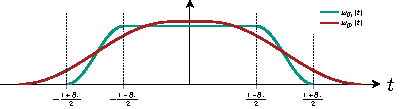
\includegraphics[width=\textwidth]{Tukey_window_TD.pdf}
         \caption{Time domain}
         \label{fig:Tukey_window_TD}
     \end{subfigure}
     \hfill
     \begin{subfigure}[b]{0.5\textwidth}
         \centering
         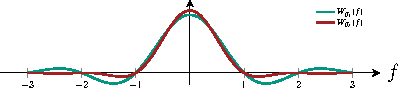
\includegraphics[width=\textwidth]{Tukey_window_FD.pdf}
         \caption{Frequency domain}
         \label{fig:Tukey_window_FD}
     \end{subfigure}
     \hfill
     \caption{Tukey window for different $\beta$, $\beta_1<\beta_2$. Based on .}
     \label{fig:Tukey_window}
\end{figure}


\end{frame}

\begin{frame}{System model}{Waveform}


\begin{figure}
\begin{center}
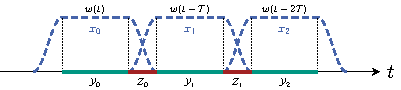
\includegraphics[width=0.9\textwidth]{Tukey_ISI.pdf}
\caption{ISI-free and ISI-pressent intervals for $n=3$. Based in .}
\label{fig:Tukey_ISI}
\end{center}
\end{figure}


\end{frame}


\begin{frame}[t]{System model}{Integrate and dump}
\begin{figure}
\begin{center}
\scalebox{0.7}{%
\begin{tikzpicture}[>=stealth,thick]%
\node [rectangle, draw, text width = 3cm, align = center, rotate=90,anchor=north] (CR) at (0,0) {Class\\Representative};
\node [rectangle, draw, text width = 3cm, align = center, rotate=90,anchor=north] (Sig) at($(CR.south)+(1,0)$) {Signaling};
\node [rectangle, draw,  text width = 3cm, align = center, rotate=90,anchor=north] (DP) at($(Sig.south)+(1,0)$) {Dispersion\\Precompensation};
\node [circle, minimum width = 0.5cm, draw, rotate=90,anchor=north] (circ1) at($(DP.south)+(1,0)$) {};
\node [circle, minimum width = 0.5cm, draw, rotate=90,anchor=north] (circ2) at($(DP.south)+(1.3,0)$) {};
\node [rectangle,  draw, text width = 3cm, align = center, rotate=90,anchor=north] (PD) at($(circ2.south)+(1,0)$) {Photodiode};
\node [rectangle, draw,kit-green100, text width = 3cm, align = center, rotate=90,anchor=north] (ID) at($(PD.south)+(1,0)$) {Integrate\\and Dump};
\node [rectangle, draw, text width = 3cm, align = center, rotate=90,anchor=north] (Det) at($(ID.south)+(1,0)$) {Detector};

\draw [->] (-1,0) -- node [above] {$k$}(CR); 
\draw [->] (CR.south) -- node [above] {$\bm x_k$} (Sig); 
\draw [->] (Sig.south) --  node [above] {$x(t)$} (DP); 
\draw [->] (DP.south) --  node [above] {$u(t)$} (circ1); 
\draw [->] (circ2.south) --  node [above] {$r(t)$} (PD); 
\draw [->] (PD.south) --  node [above] {$s(t)$} (ID); 
\draw [->] (ID.south) --  node [above] {$\bm y,\bm z$}(Det); 
\draw [->] (Det.south) -- node [above] {$\hat{k}$}+ (1,0);



\end{tikzpicture}

}
\end{center}
\end{figure}


This block integrates the incoming signal $s(t)$ in the different intervals $\mathcal{Y}_i$ and $\mathcal{Z}_i$ to produce the real valued samples $y_i$ and $z_i$ given by:
\begin{align}
	y_i&=\int_{\mathcal Y_i}s(t)dt&&i\in \{0,\dotsc,n-1\}\\
	z_i&=\int_{\mathcal Z_i}s(t)dt&&i\in \{0,\dotsc,n-2\}
\end{align}



\end{frame}

\begin{frame}{System model}{Integrate and dump}

It can be shown that $y_i$ is given by :
\begin{equation}
y_i=\alpha^2(1-\beta)T|x_i|^2+\alpha|x_i|n_i+m_i
	\label{eq:y_i_Tukey}
\end{equation}
where $\alpha=2/\sqrt{4-\beta}$, $n_i\sim\mathcal N(0,\sigma^2_{sh}(1-\beta)T)$ and $m_i\sim\mathcal N(0,\sigma^2_{th}(1-\beta)T)$.%

And that $z_i$ is given by :
\begin{equation}
	z_i=\alpha^2\beta T\psi(x_i,x_{i+1})+\alpha\sqrt{\psi(x_i,x_{i+1})}p_i +q_i
	\label{eq:z_i_Tukey}
\end{equation}
where $p_i\sim\mathcal N(0,\sigma^2_{sh}\beta T)$ and $q_i\sim\mathcal N(0,\sigma^2_{th}\beta T)$, and 
\begin{align}
\psi(ae^{j\alpha},be^{j\beta})&=\frac{3}{8}\left(a^2+b^2\right)+\frac{1}{4}ab\cos(\alpha-\beta)
\end{align}



\end{frame}


\begin{frame}{System model}{Class representative}

\begin{figure}
\begin{center}
\scalebox{0.7}{%
\begin{tikzpicture}[>=stealth,thick]%
\node [rectangle, draw, kit-green100,text width = 3cm, align = center, rotate=90,anchor=north] (CR) at (0,0) {Class\\Representative};
\node [rectangle, draw, text width = 3cm, align = center, rotate=90,anchor=north] (Sig) at($(CR.south)+(1,0)$) {Signaling};
\node [rectangle, draw,  text width = 3cm, align = center, rotate=90,anchor=north] (DP) at($(Sig.south)+(1,0)$) {Dispersion\\Precompensation};
\node [circle, minimum width = 0.5cm, draw, rotate=90,anchor=north] (circ1) at($(DP.south)+(1,0)$) {};
\node [circle, minimum width = 0.5cm, draw, rotate=90,anchor=north] (circ2) at($(DP.south)+(1.3,0)$) {};
\node [rectangle,  draw, text width = 3cm, align = center, rotate=90,anchor=north] (PD) at($(circ2.south)+(1,0)$) {Photodiode};
\node [rectangle, draw, text width = 3cm, align = center, rotate=90,anchor=north] (ID) at($(PD.south)+(1,0)$) {Integrate\\and Dump};
\node [rectangle, draw, text width = 3cm, align = center, rotate=90,anchor=north] (Det) at($(ID.south)+(1,0)$) {Detector};

\draw [->] (-1,0) -- node [above] {$k$}(CR); 
\draw [->] (CR.south) -- node [above] {$\bm x_k$} (Sig); 
\draw [->] (Sig.south) --  node [above] {$x(t)$} (DP); 
\draw [->] (DP.south) --  node [above] {$u(t)$} (circ1); 
\draw [->] (circ2.south) --  node [above] {$r(t)$} (PD); 
\draw [->] (PD.south) --  node [above] {$s(t)$} (ID); 
\draw [->] (ID.south) --  node [above] {$\bm y,\bm z$}(Det); 
\draw [->] (Det.south) -- node [above] {$\hat{k}$}+ (1,0);



\end{tikzpicture}

}
\end{center}
\end{figure}


When transmitting symbol blocks (n consecutive symbols), it turns out that there are some ambiguities, which means that two different symbol blocks produce the same output of the system. Of course, we want to avoid this situation to achieve reliable communication. That is what the Class representative block does.

\end{frame}

\begin{frame}[t]{System model}{Class representative}
let define the function $\Upsilon: \mathds{C}^n\to(\mathds{R}^n,\mathds{R}^{n-1})$ that maps a vector $\bm x$ at the input of the signaling block, to the output of the integrate and dump block, in the absence of noise. That means:
\begin{align}
	\Upsilon(\bm x) = (\bm y, \bm z)
\end{align}
where $\bm x\in\mathds{C}^n$, $\bm y\in\mathds{R}^n$, $\bm z\in\mathds{R}^{n-1}$ and 
\begin{align}
	y_i&=\int_{\mathcal Y_i}\bigl|x(t)\bigr|^2dt&&i\in \{0,\dotsc,n-1\}\\
	z_i&=\int_{\mathcal Z_i}\bigl|x(t)\bigr|^2dt&&i\in \{0,\dotsc,n-2\}
\end{align}

Now we define an equivalence relation in $\mathds C^n$, where two vectors $\bm x$ and $\bm{\tilde{x}}$ are square law equivalent if and only if $\Upsilon(\bm x)=\Upsilon(\bm{\tilde{x}})$, and we denote the equivalence by $\bm x \equiv \bm{\tilde{x}}$.

\end{frame}



\begin{frame}{System model}{Class representative}
		\begin{greenblock}{Class representative}

The Class representative block consist of a set $\mathcal S$ of cardinality $M$, whose elements belong to $\mathds{C}^n$ and are all square law distinct, that is:
\begin{align}
	\mathcal S = \{\bm x_1, \dotsc,\bm x_M\} \subset\mathds C^n\qquad \text{such that}\qquad\bm x_i\not\equiv\bm x_l \Leftrightarrow k\neq l
\end{align}
and for an input $k\in\{1,\dotsc,M\}$ the block outputs $\bm x_k$:
\end{greenblock}

\begin{greenblock}{Equivalence class}
Let us define equivalence class as the set of all vectors, that are equivalent, so an equivalence class $\mathcal{E}$ of size $L$ is given by:
\begin{align}
	\mathcal E=\{\bm x_1, \dotsc,\bm x_L\} \subset\mathcal K^n\qquad \text{such that}\qquad\bm x_i\equiv\bm x_j\quad \forall i,j \in \{1,\dotsc,L\} 
\end{align}

\end{greenblock}

\end{frame}

\begin{frame}{System model}{Ambiguities}
\begin{figure}[hub]
     \centering
     \begin{subfigure}[b]{0.4\textwidth}
         \centering
         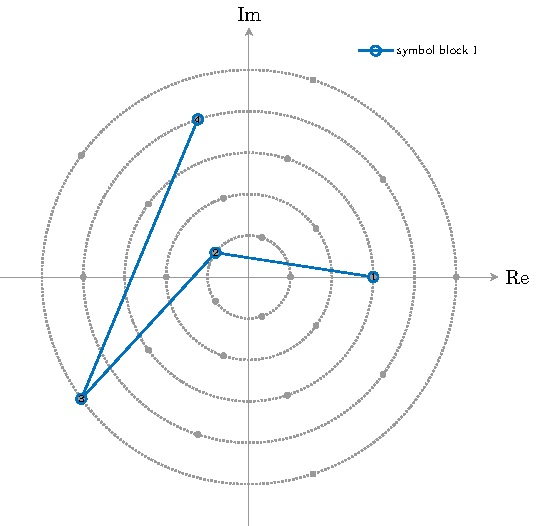
\includegraphics[width=\textwidth]{Eq_class_construction_0.pdf}
     \end{subfigure}
     \hspace{10mm}
     \begin{subfigure}[b]{0.4\textwidth}
         \centering
         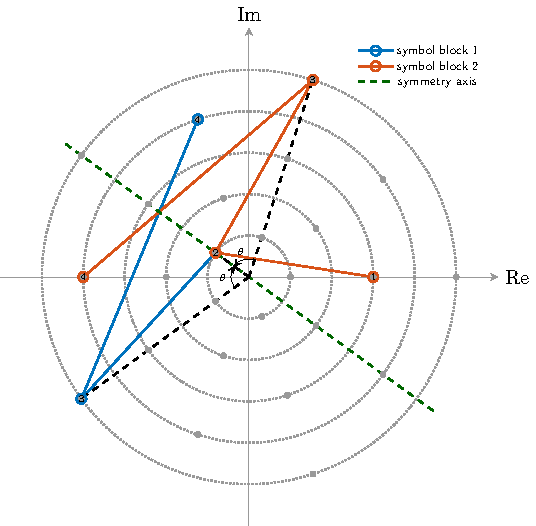
\includegraphics[width=\textwidth]{Eq_class_construction_1.pdf}
     \end{subfigure}
\end{figure}

\end{frame}

\begin{frame}{System model}{Ambiguities}
\begin{figure}[htb]
     \centering
     \begin{subfigure}[b]{0.4\textwidth}
         \centering
         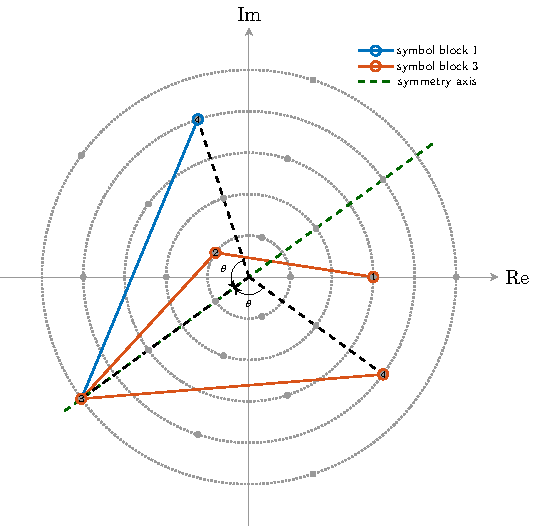
\includegraphics[width=\textwidth]{Eq_class_construction_2.pdf}
     \end{subfigure}
     \hspace{10mm}
     \begin{subfigure}[b]{0.4\textwidth}
         \centering
         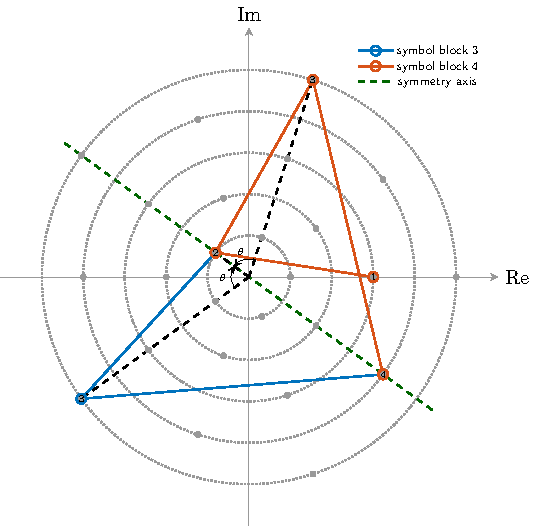
\includegraphics[width=\textwidth]{Eq_class_construction_3.pdf}
     \end{subfigure}
\end{figure}

\end{frame}
\begin{frame}{System model}{Ambiguities}
\begin{figure}[htb]
     \centering
     \begin{subfigure}[b]{0.4\textwidth}
         \centering
         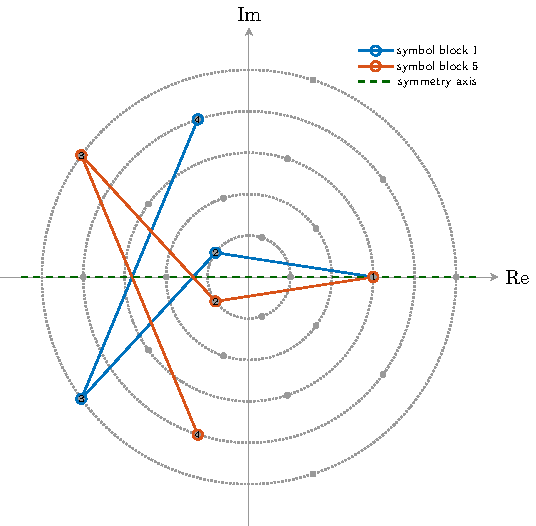
\includegraphics[width=\textwidth]{Eq_class_construction_4.pdf}
     \end{subfigure}
     \hspace{10mm}
     \begin{subfigure}[b]{0.4\textwidth}
         \centering
         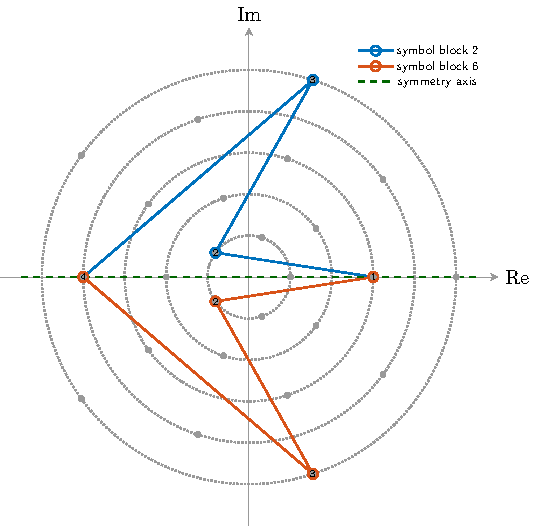
\includegraphics[width=\textwidth]{Eq_class_construction_5.pdf}
     \end{subfigure}
\end{figure}

\end{frame}
\begin{frame}{System model}{Ambiguities}
\begin{figure}[htb]
     \centering
     \begin{subfigure}[b]{0.4\textwidth}
         \centering
         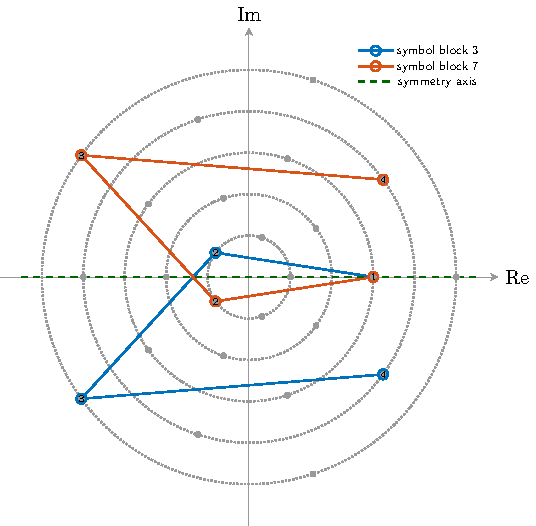
\includegraphics[width=\textwidth]{Eq_class_construction_6.pdf}
     \end{subfigure}
     \hspace{10mm}
     \begin{subfigure}[b]{0.4\textwidth}
         \centering
         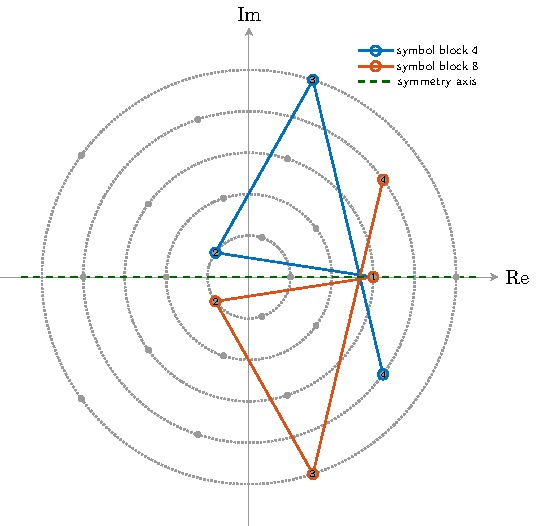
\includegraphics[width=\textwidth]{Eq_class_construction_7.pdf}
     \end{subfigure}
\end{figure}

\end{frame}
\begin{frame}{System model}{Ambiguities}
\begin{figure}[htb]
     \centering
     \begin{subfigure}[b]{0.4\textwidth}
         \centering
         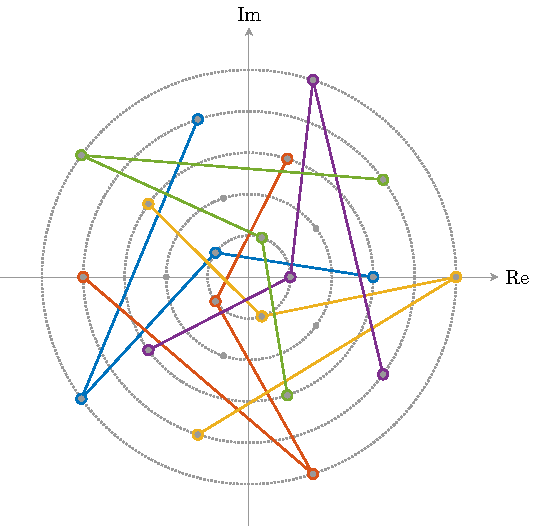
\includegraphics[width=\textwidth]{Eq_class_construction_8.pdf}
     \end{subfigure}
     \hspace{10mm}
     \begin{subfigure}[b]{0.4\textwidth}
         \centering
         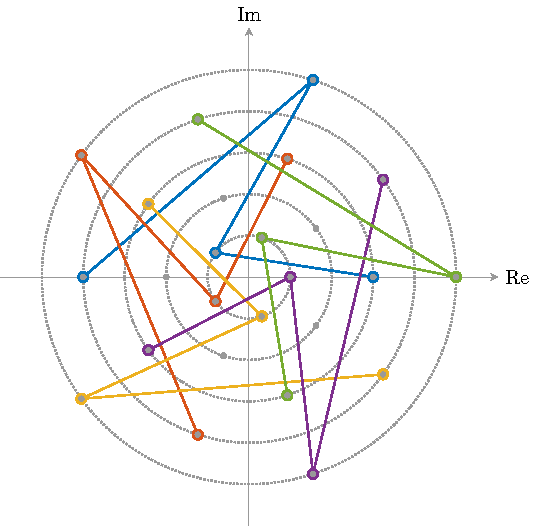
\includegraphics[width=\textwidth]{Eq_class_construction_9.pdf}
     \end{subfigure}
\end{figure}

\end{frame}
\begin{frame}{System model}{Ambiguities}
\begin{figure}[htb]
     \centering
     \begin{subfigure}[b]{0.4\textwidth}
         \centering
         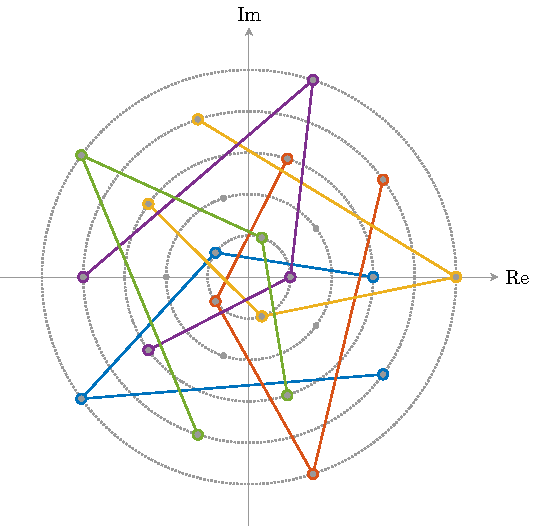
\includegraphics[width=\textwidth]{Eq_class_construction_10.pdf}
     \end{subfigure}
     \hspace{10mm}
     \begin{subfigure}[b]{0.4\textwidth}
         \centering
         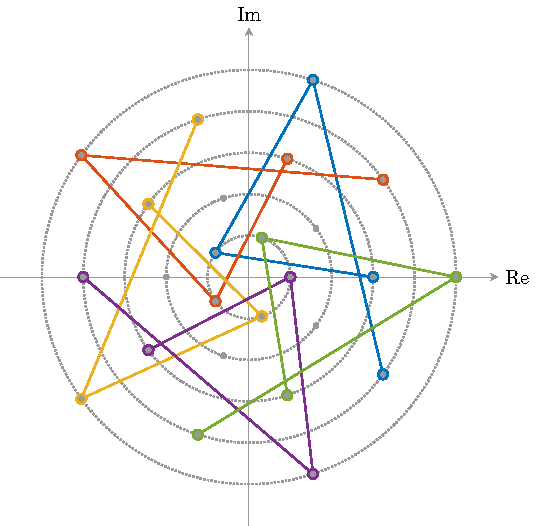
\includegraphics[width=\textwidth]{Eq_class_construction_11.pdf}
     \end{subfigure}
\end{figure}

\end{frame}
\begin{frame}{System model}{Ambiguities}
\begin{figure}[htb]
     \centering
     \begin{subfigure}[b]{0.4\textwidth}
         \centering
         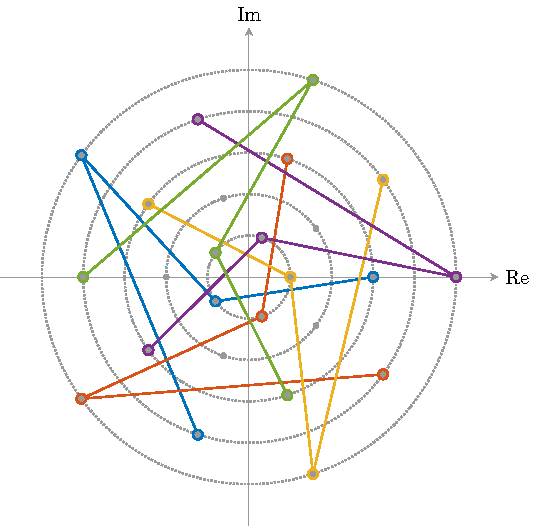
\includegraphics[width=\textwidth]{Eq_class_construction_12.pdf}
     \end{subfigure}
     \hspace{10mm}
     \begin{subfigure}[b]{0.4\textwidth}
         \centering
         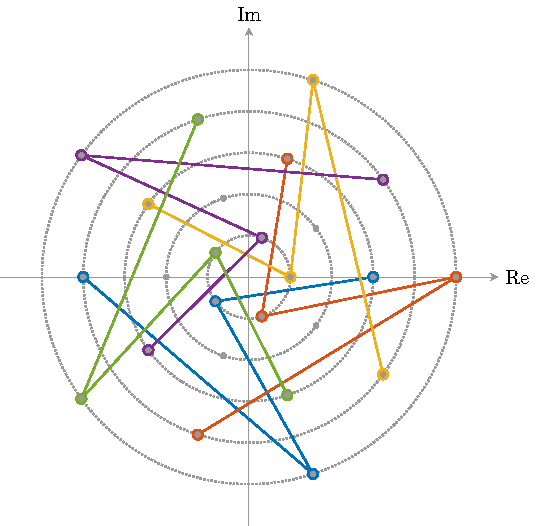
\includegraphics[width=\textwidth]{Eq_class_construction_13.pdf}
     \end{subfigure}
\end{figure}

\end{frame}
\begin{frame}{System model}{Ambiguities}
\begin{figure}[htb]
     \centering
     \begin{subfigure}[b]{0.4\textwidth}
         \centering
         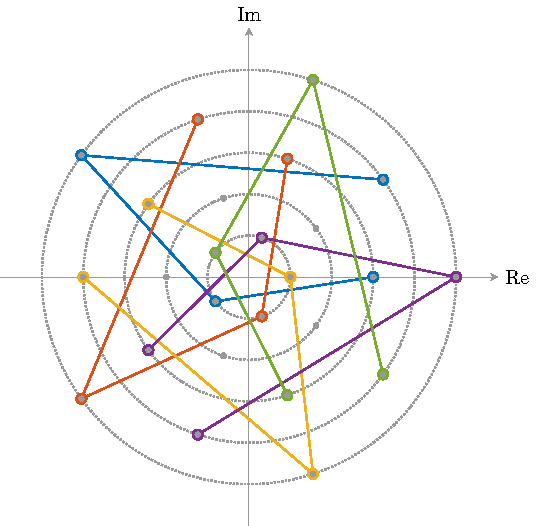
\includegraphics[width=\textwidth]{Eq_class_construction_14.pdf}
     \end{subfigure}
     \hspace{10mm}
     \begin{subfigure}[b]{0.4\textwidth}
         \centering
         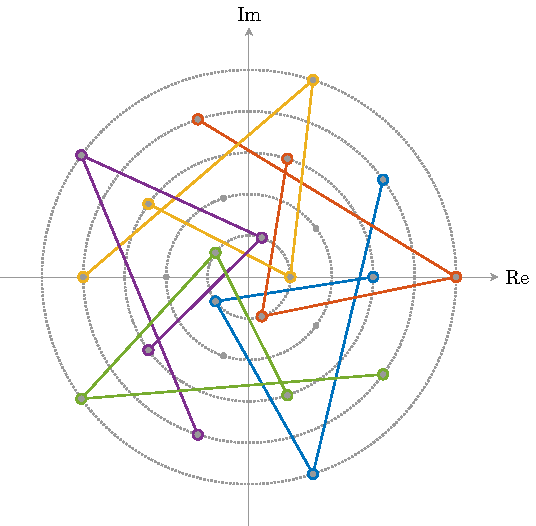
\includegraphics[width=\textwidth]{Eq_class_construction_15.pdf}
     \end{subfigure}
\end{figure}

\end{frame}
\begin{frame}{System model}{Ambiguities}
\begin{figure}[htb]
     \centering
         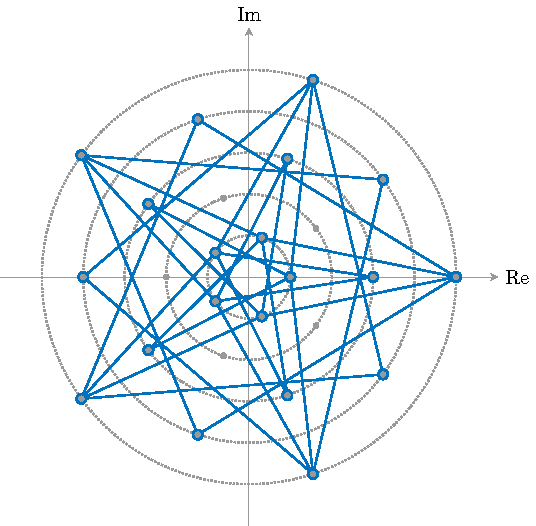
\includegraphics[height=0.7\textheight]{Eq_class_construction_16.pdf}
\end{figure}

\end{frame}



\begin{frame}{System model}{Detector}

\begin{figure}
\begin{center}
\scalebox{0.7}{%
\begin{tikzpicture}[>=stealth,thick]%
\node [rectangle, draw, text width = 3cm, align = center, rotate=90,anchor=north] (CR) at (0,0) {Class\\Representative};
\node [rectangle, draw, text width = 3cm, align = center, rotate=90,anchor=north] (Sig) at($(CR.south)+(1,0)$) {Signaling};
\node [rectangle, draw,  text width = 3cm, align = center, rotate=90,anchor=north] (DP) at($(Sig.south)+(1,0)$) {Dispersion\\Precompensation};
\node [circle, minimum width = 0.5cm, draw, rotate=90,anchor=north] (circ1) at($(DP.south)+(1,0)$) {};
\node [circle, minimum width = 0.5cm, draw, rotate=90,anchor=north] (circ2) at($(DP.south)+(1.3,0)$) {};
\node [rectangle,  draw, text width = 3cm, align = center, rotate=90,anchor=north] (PD) at($(circ2.south)+(1,0)$) {Photodiode};
\node [rectangle, draw, text width = 3cm, align = center, rotate=90,anchor=north] (ID) at($(PD.south)+(1,0)$) {Integrate\\and Dump};
\node [rectangle, draw, kit-green100,text width = 3cm, align = center, rotate=90,anchor=north] (Det) at($(ID.south)+(1,0)$) {Detector};

\draw [->] (-1,0) -- node [above] {$k$}(CR); 
\draw [->] (CR.south) -- node [above] {$\bm x_k$} (Sig); 
\draw [->] (Sig.south) --  node [above] {$x(t)$} (DP); 
\draw [->] (DP.south) --  node [above] {$u(t)$} (circ1); 
\draw [->] (circ2.south) --  node [above] {$r(t)$} (PD); 
\draw [->] (PD.south) --  node [above] {$s(t)$} (ID); 
\draw [->] (ID.south) --  node [above] {$\bm y,\bm z$}(Det); 
\draw [->] (Det.south) -- node [above] {$\hat{k}$}+ (1,0);



\end{tikzpicture}

}
\end{center}
\end{figure}

For the detection, the maximum-likelihood (ML) criterion is chosen:
\begin{equation}
\hat{k}=\argmax_{d\in\{1,\dotsc,M\}}f\bigl(\bm y,\bm z|\bm x_d\bigr)
\label{eq:Tukey_ML}
\end{equation}

Where the PDF of $\bm y,\bm z$ given $\bm x_d$ is given by :%
\begin{equation}
	f\bigl(\bm y,\bm z|\bm x_d\bigr) = f\bigl(\bm y|\bm x_d\bigr)f\bigl(\bm z|\bm x_d\bigr)=\prod_{i=0}^{n-1}f\bigl(y_i|\bm x_d[i]\bigr)\prod_{i=0}^{n-2}f\bigl(z_i|\bm x_d[i],\bm x_d[i+1]\bigr)
\end{equation}



\end{frame}

\subsection{Numerical simulation}

\begin{frame}{Numerical simulation}{Simulation for a 2-ring 4-ary constellation}
\begin{table}[!ht]
\begin{center}
\begin{tabular}{|r|m{10mm}<{\raggedleft}|m{10mm}<{\raggedleft}|m{10mm}<{\raggedleft}|m{10mm}<{\raggedleft}|m{10mm}<{\raggedleft}|}\hline
\backslashbox{Class size}{Block length}&3&4&5&6&7\\\hline
4&32&128&512&2048&8192\\
8&32&192&1024&5120&24576\\
16&8&96&768&5120&30720\\
32&&16&256&2560&20480\\
64&&&32&640&7680\\
128&&&&64&1536\\
256&&&&&128\\\hline
Total&72&432&2592&15552&93312\\\hline
Rate loss (bit/sym)&0.94&0.81&0.73&0.68&0.64\\\hline
\end{tabular}
\end{center}
\caption{Number of equivalence classes for 2-ring 4-ary Phase constellation.}
\label{tab:Eq_class_2ring_4ary}
\end{table}%

\end{frame}

\begin{frame}{Numerical simulation}{Simulation for a 2-ring 4-ary constellation}
\begin{figure}
\begin{center}
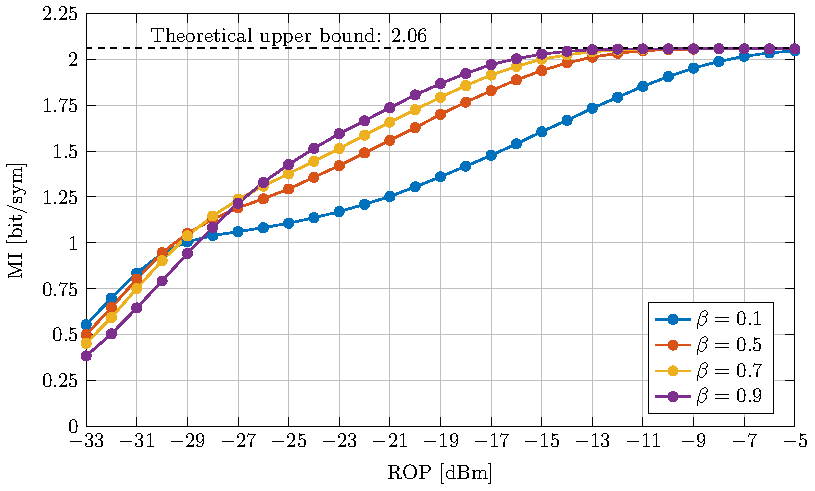
\includegraphics[width=0.6\textwidth]{Tukey_result_MI.pdf}
\caption{Mutual information of the system with 2-ring 4-ary phase constellation and symbol block length $n=3$.}
\label{fig:Tukey_result_MI}
\end{center}
\end{figure}

\end{frame}


\begin{frame}{Numerical simulation}{Simulation for a 2-ring 4-ary constellation}
\begin{figure}
\begin{center}
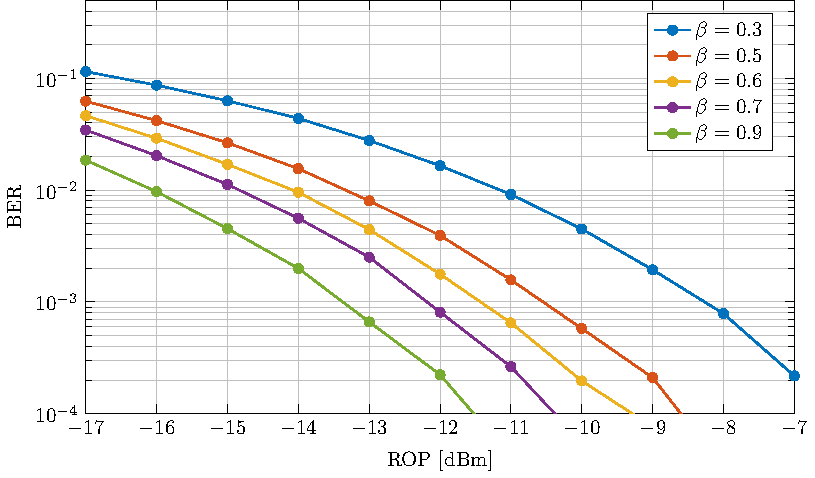
\includegraphics[width=0.6\textwidth]{Tukey_result_BER.pdf}
\caption{Bit error rate of the system with 2-ring 4-ary phase constellation and symbol block length $n=4$.}
\label{fig:Tukey_result_BER}
\end{center}
\end{figure}

\end{frame}



\subsection{Discussion}


\begin{frame}{Discussion}{}
\begin{greenblock}{Disadvantages}
		
\begin{itemize}

\item \textbf{The complexity of the decoder}: To decrease the rate loss the block length must increase, but the complexity grows exponentially with the block length.
\item \textbf{The bandwidth efficiency}: Tukey window is a time limited signal, hence its spectrum is wide, so the bandwidth efficiency is bad.
\item \textbf{The implementation}: The integrate and dump block is an analog and hence may be difficult to implement.

\end{itemize}
\end{greenblock}
		
\end{frame}



%%%%%%%%%%%%%%%%%%%%%%%%%%%%%%%%%%%%%
\section[Generalized direct detection]{Generalized direct detection with phase recovery}

\begin{frame}{}{}
\center\Huge Generalized direct detection with phase recovery
\end{frame}


\subsection{System model}

\begin{frame}{System model}{}
\begin{figure}
\begin{center}
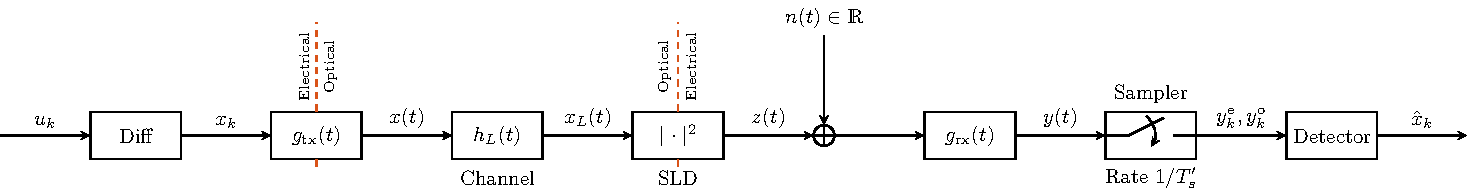
\includegraphics[width=\textwidth]{Plabst_system_model.pdf}
\end{center}
\end{figure}
\end{frame}


\begin{frame}{System model}{Differential encoder}

The phase encoding is done by a function that receives as an input a vector of symbols $\bm u$ and outputs a vector of symbols $\bm x=f_\text{diff}(\bm u)$ with the same magnitude as the symbols in $\bm u$, and a given phase based on a set of conditions

\begin{figure}[htbp]
\begin{center}
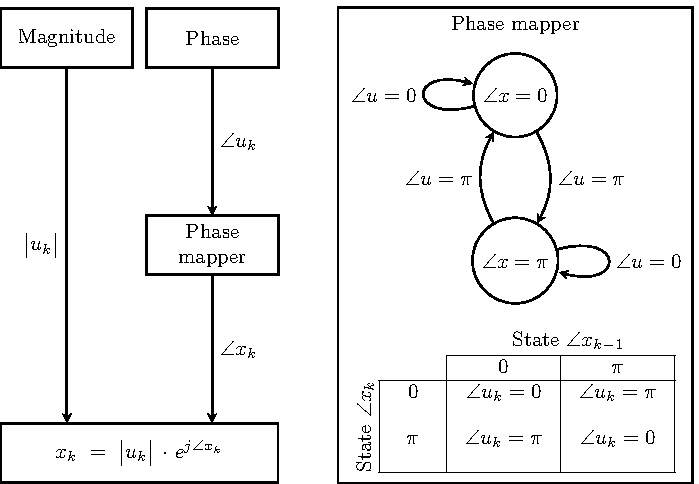
\includegraphics[width=0.4\textwidth]{diff_map_M_ASK.pdf}
\caption{Differential phase mapper example for M-ASK.}
\label{fig:diff_encoding}
\end{center}
\end{figure}


\end{frame}

\begin{frame}{System model}{Transmitter}

The transmitter receives as input a sequence $\bm x=\{x_0,\dotsc,x_{n-1}\}$ of independent and identically distributed (i.i.d.) symbols $x_i$ taken from a finite constellation $\mathcal K=\{a_1,\dotsc,a_q\}$ with $q$ elements, and outputs a signal given by:%
\begin{equation}
x(t)=\sum_{k=0}^{n-1}x_k\cdot g_\text{tx}(t-iT)
\label{eq:Plabst_signaling_block}
\end{equation}
where $T$ is the inverse of the symbol rate, $x_i\in\mathcal K$, and $g_\text{tx}(t)$ is the pulse waveform.

\end{frame}

\begin{frame}{System model}{Transmission medium and receiver}
The channel considered is an optic fiber that only presents chromatic dispersion, characterized in the frequency domain by:
\begin{equation}
H_L(f)=e^{j2\beta_2L\pi^2f^2}
\end{equation}
where $\beta_2$ is the group-velocity dispersion parameter and $L$ is the fiber length.

The receiver consists of a photodiode, whose output is given by:
\begin{equation}
z(t)=|x_L(t)|^2
\end{equation}

\end{frame}


\begin{frame}{System model}{sampler}
For the sample an oversampling factor of $N_\text{os}=T_s/T'_s=2$ is used. Let $\bm x'=\{0,x_0,\dotsc0,x_{n-1}\}$ and $\bm y'=\{y_0,\dotsc,y_{2n-1}\}$ be the upsampled sequence at the transmitter and receiver.
\begin{align}
y'_k&=z'_k+n'_k \\
z'_k&=\left(|x_L(t)|^2*g_\text{rx}(t)\right)_{t=kT'_s}
\end{align}
where $n_k\sim\mathcal N(0,\sigma_N^2)$ and $\sigma_N^2=N_0B$.

Now let us define the combined impulse response as $\uppsi(t)=g_\text{tx}(t)*h_L(t)$ and the discrete version of it $\uppsi_k=\uppsi(kT'_s)$, then:
\begin{equation}
x_L(kT'_s)=\sum_{m=0}^{2n-1}\uppsi_mx'_{k-m}
\end{equation}


\end{frame}

\begin{frame}{System model}{sampler}

Finally, if the pulse shape is a sinc pulse, $|x_L(t)|^2*g_\text{rx}=|x_L(t)|^2$, so:
\begin{equation}
z'_k=\left|\sum_{m=0}^{2n-1}\uppsi_mx'_{k-m}\right|^2
\end{equation}
 
Which can be expressed in vector matrix notation if we define the Toeplitz matrix $\bm \Uppsi$ and the channel state $\bm{s}'_0=[0,x_{-\widetilde{M}},0,x_{1-\widetilde{M}},\dotsc,0,x_{-1}]^T$ as:
\begin{align}
	\bm y' = \left|\bm \Uppsi \left[
\begin{array}{c}
\bm{s}'_0  \\
   \bm x'
\end{array}
\right]
\right|^{\circ2} + \bm n' = \left|\bm{ \Uppsi \tilde{x'}}\right|^{\circ2} +\bm n' \qquad \in \mathds{R}^{2n}
\end{align}


\end{frame}


\begin{frame}{System model}{Even and odd samples}

\begin{figure}[htbp]
\begin{center}
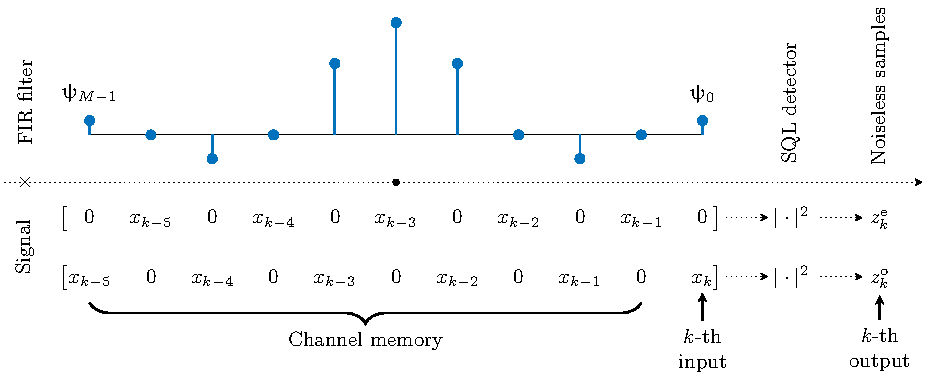
\includegraphics[width=0.75\textwidth]{Exp_even_odd_samp.pdf}
\end{center}
\end{figure}


\begin{align}
&\bm z_k= \bigl[z'_{2k},z'_{2k+1}\bigr]=\bigl[z_{k}^{\text{e}},z_{k}^{\text{o}}\bigr]
&&\bm y_k=\bigl[y_{k}^{\text{e}},y_{k}^{\text{o}}\bigr]=\bm z_k+\bigl[n_{k}^{\text{e}}, n_{k}^{\text{o}}\bigr]
\end{align}


\end{frame}


\begin{frame}{System model}{Symbol-wise MAP detection}

\begin{align}
\hat{x}_k=\argmax_{x_k}p(x_k,\bm y')
p(x_k,\bm y')=\sum_{s_0}\sum_{\bm x\backslash x_k} p(s_0,\bm x, \bm y')
\label{eq:APPs}
\end{align}
and $\sum_{\bm x\backslash x_k}$ denotes a sum over all possible vectors $\bm x$  but where the $k$-th position is fixed.


\begin{figure}[htbp]
\begin{center}
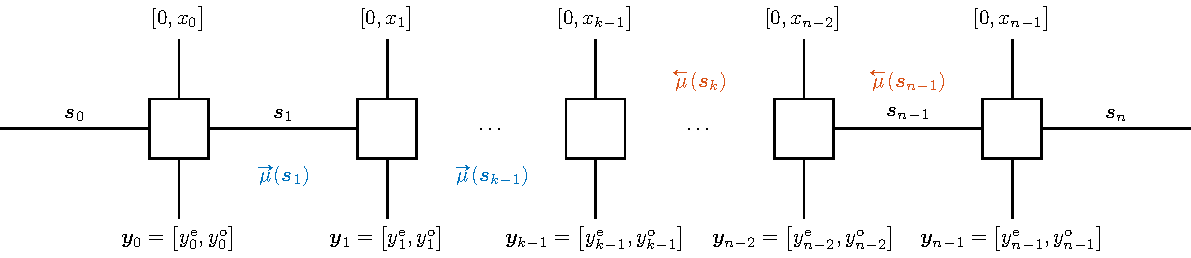
\includegraphics[width=0.8\textwidth]{BCJR.pdf}
\end{center}
\end{figure}
\end{frame}


\subsection{Numerical simulation}

\begin{frame}{Numerical simulation}{Auxiliary channel}

\begin{figure}[htbp]
\begin{center}
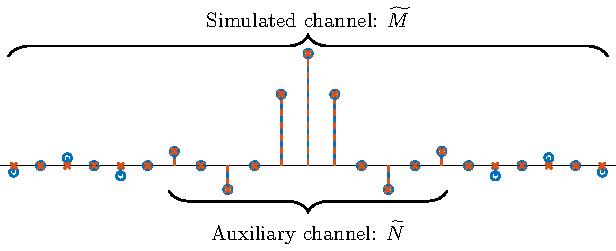
\includegraphics[width=0.8\textwidth]{aux_channel.pdf}
\end{center}
\end{figure}


\end{frame}


\begin{frame}{Numerical simulation}{Constellations}

For the simulation we used BPSK, QAM, and a specially designe constellation, named DD-SQAM.

\begin{figure}[!ht]
\begin{center}
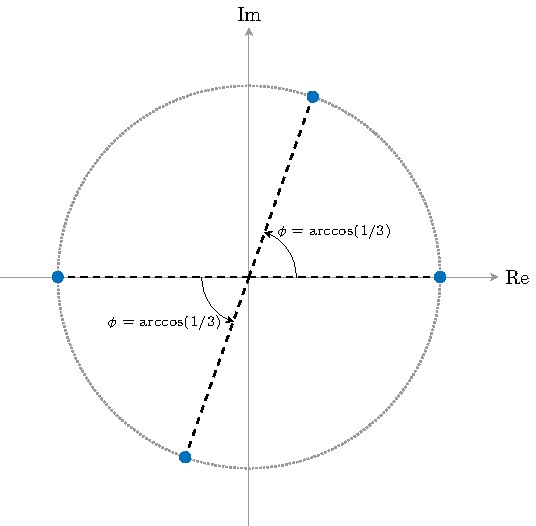
\includegraphics[width=0.4\textwidth]{DD_SQAM_constellation.pdf}
\end{center}
\end{figure}


\end{frame}

\begin{frame}{Numerical simulation}{Results}
\begin{figure}[!ht]
\begin{center}
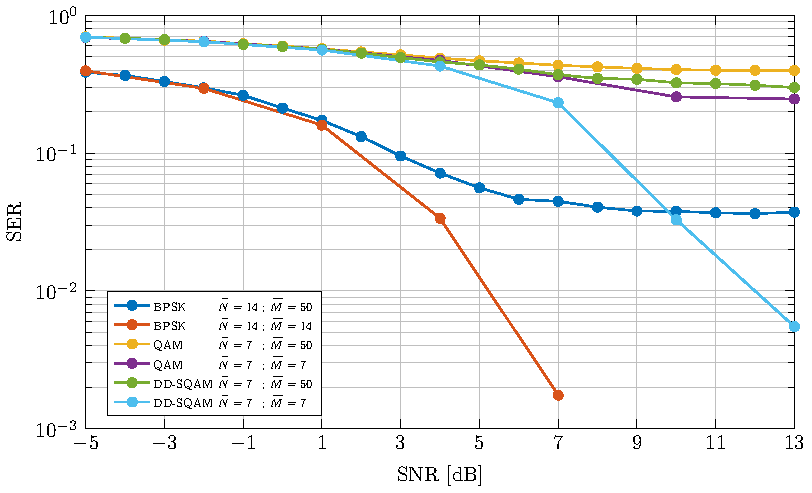
\includegraphics[width=0.6\textwidth]{Plabst_result_SER.pdf}
\end{center}
\end{figure}

\end{frame}


\subsection{Discussion}

\begin{frame}{Discussion}

\begin{itemize}
\item The system is more flexible, since the waveform have no restriction.
\item The spectral efficiency is better than in the previous system.
\item The system has an oversampling of only 2.
\item The decoder is still to complex to be feasible.
\end{itemize}


\end{frame}

%%%%%%%%%%%%%%%%%%%%%%%%%%%%%%%%%%%%%
\section{MagPhase-DetNet}

\begin{frame}{}{}
\center\Huge MagPhase-DetNet
\end{frame}


\subsection{Architecture}

\begin{frame}{Architecture}
\begin{figure}[htb]
     \centering
	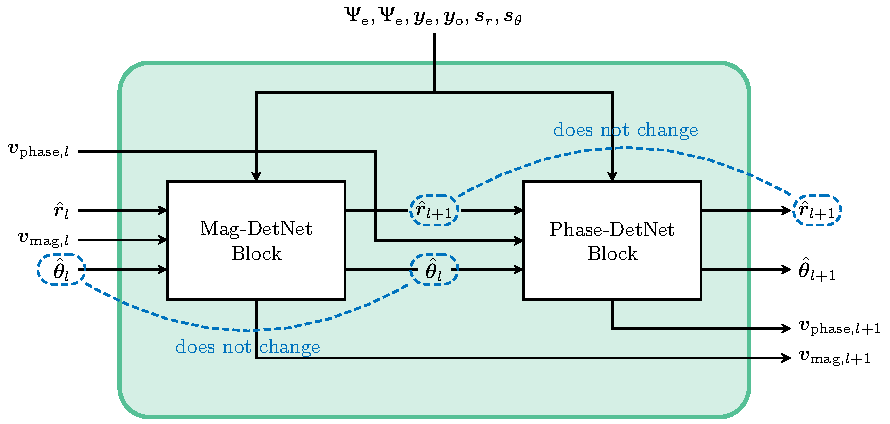
\includegraphics[width=0.8\textwidth]{magPhaseDetNet_block.pdf}
\end{figure}

\end{frame}

\begin{frame}{Architecture}
\begin{figure}[htb]
         \centering
         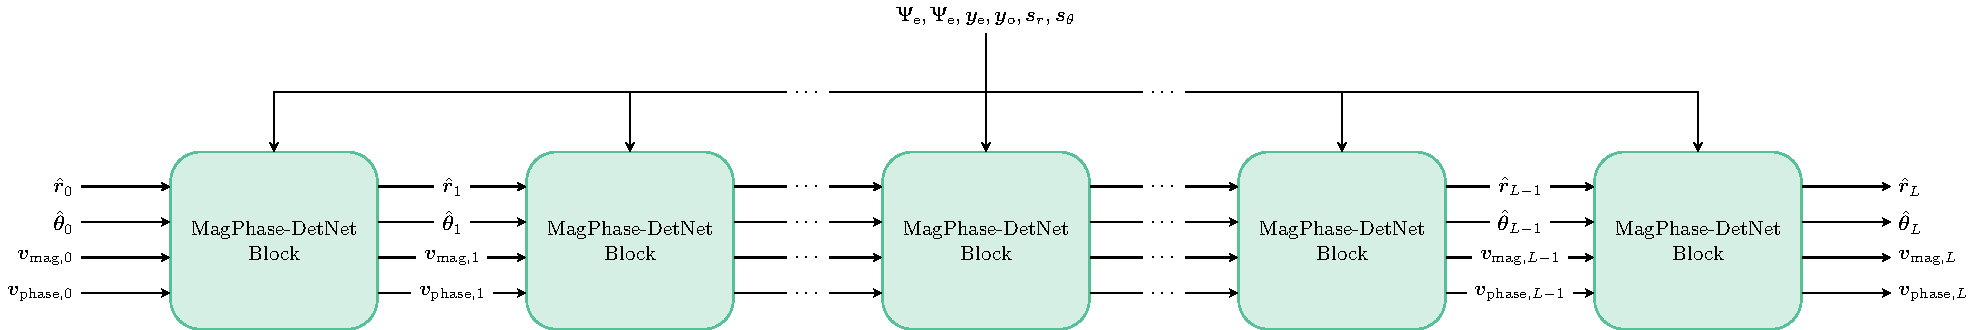
\includegraphics[width=0.95\textwidth]{magPhaseDetNet_architecture.pdf}
\end{figure}

\end{frame}

\subsection{Numerical simulation}

\begin{frame}{Numerical simulation}{Training process}

For the training we use a variable batch size that takes the following values in order $[100, 400, 1000, 2000, 5000, 10000]$ and performs 300 learning processes for each batch size.

\begin{figure}[!ht]
\begin{center}
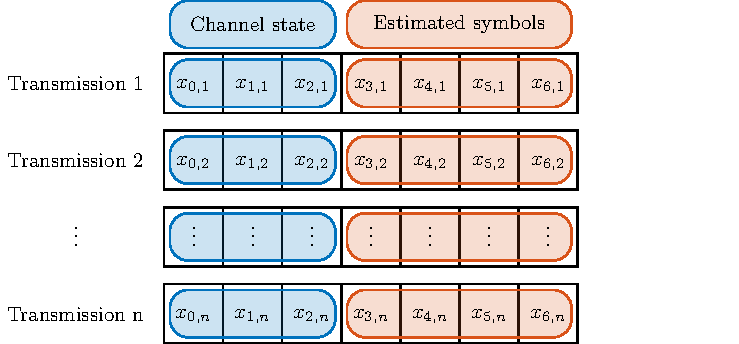
\includegraphics[width=0.6\textwidth]{train_normal.pdf}
\end{center}
\end{figure}

\end{frame}


\begin{frame}{Numerical simulation}{Evaluation process}

\begin{figure}[!ht]
\begin{center}
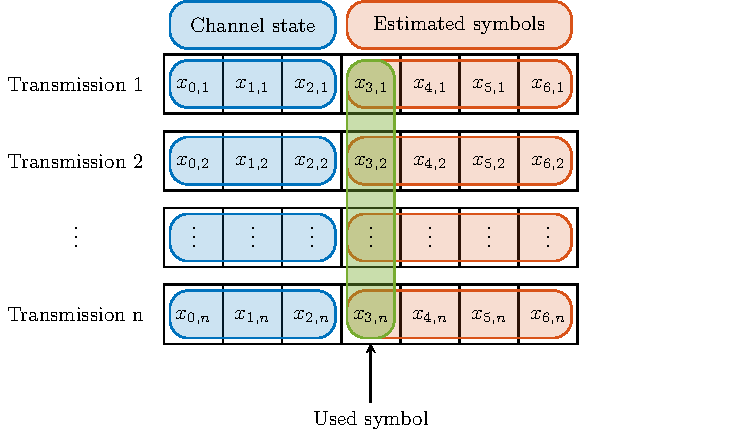
\includegraphics[width=0.6\textwidth]{eval_normal.pdf}
\end{center}
\end{figure}

\end{frame}


\begin{frame}{Numerical simulation}{Evaluation process}

\begin{figure}[!ht]
\begin{center}
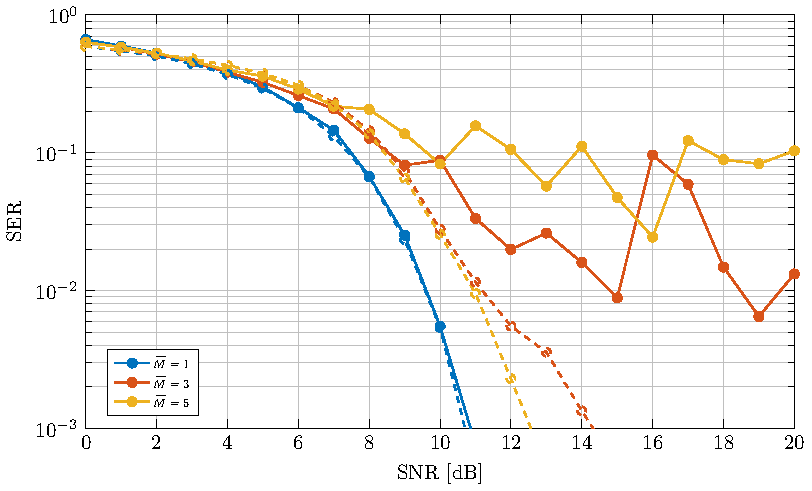
\includegraphics[width=0.6\textwidth]{SER_normal_test.pdf}
\end{center}
\end{figure}
\end{frame}


\begin{frame}{Numerical simulation}{Evaluation process}

\begin{figure}[!ht]
\begin{center}
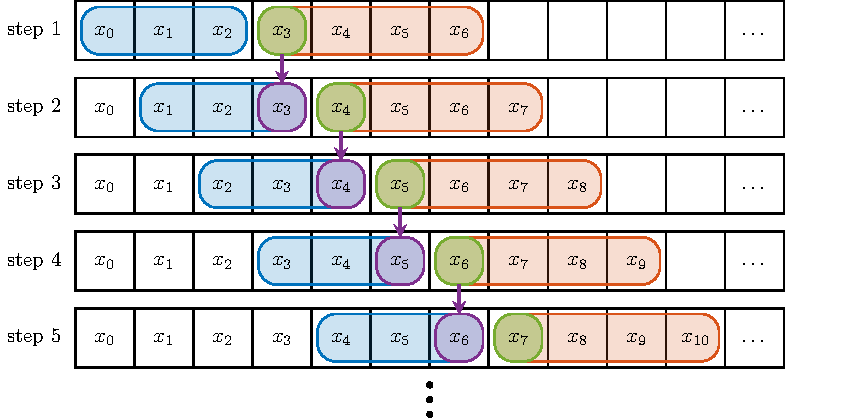
\includegraphics[width=0.65\textwidth]{eval_seq.pdf}
\end{center}
\end{figure}

\end{frame}


\begin{frame}{Numerical simulation}{Evaluation process}

\begin{figure}[!ht]
\begin{center}
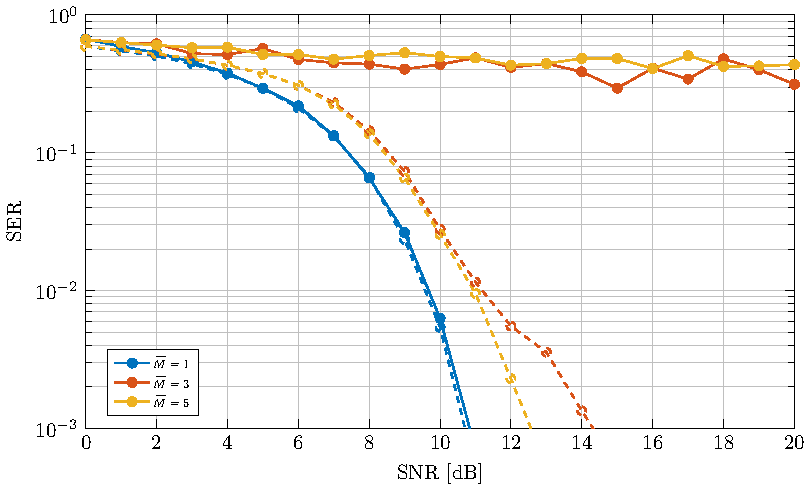
\includegraphics[width=0.6\textwidth]{SER_seq_test.pdf}
\end{center}
\end{figure}
\end{frame}



\subsection{Conclussions}

\begin{frame}{Conclussions}

\begin{itemize}
\item The trained MagPhase-DetNet network's performance is not as good as needed because the trained models present a high error floor.
\item When trying the sequential evaluation the bad performance shows that the architecture is not the most adequate, may be a conventional approach could be better.
\item The training process seems to be slower for longer channel memory.
\end{itemize}








\end{frame}


\appendix
\beginbackup

\begin{frame}[allowframebreaks]{References}
\nocite{*}
\printbibliography
\end{frame}



%
%\begin{frame}{Blöcke}{in den KIT-Farben}
%	\begin{columns}
%		\column{.3\textwidth}
%		\begin{greenblock}{Greenblock}
%			Standard (\texttt{block})
%        \end{greenblock}
%		\column{.3\textwidth}
%		\begin{blueblock}{Blueblock}
%			= \texttt{exampleblock}
%        \end{blueblock}
%		\column{.3\textwidth}
%		\begin{redblock}{Redblock}
%			= \texttt{alertblock}
%        \end{redblock}
%	\end{columns}
%	\begin{columns}
%		\column{.3\textwidth}
%        \begin{brownblock}{Brownblock}
%        \end{brownblock}
%		\column{.3\textwidth}
%        \begin{purpleblock}{Purpleblock}
%        \end{purpleblock}
%		\column{.3\textwidth}
%        \begin{cyanblock}{Cyanblock}
%        \end{cyanblock}
%	\end{columns}
%	\begin{columns}
%		\column{.3\textwidth}
%        \begin{yellowblock}{Yellowblock}
%        \end{yellowblock}
%		\column{.3\textwidth}
%        \begin{lightgreenblock}{Lightgreenblock}
%        \end{lightgreenblock}
%		\column{.3\textwidth}
%        \begin{orangeblock}{Orangeblock}
%        \end{orangeblock}
%	\end{columns}
%	\begin{columns}
%		\column{.3\textwidth}
%        \begin{grayblock}{Grayblock}
%        \end{grayblock}
%		\column{.3\textwidth}
%		\begin{contentblock}{Contentblock}
%			(farblos)
%		\end{contentblock}
%		\column{.3\textwidth}
%	\end{columns}
%\end{frame}
%	  
%%
%
%%% ----------------------------------------
%%% | Test-Folie mit definierten Farben |
%%% ----------------------------------------
%\begin{frame}{Farbpalette}
%\tiny
%
%% GREEN
%	\colorbox{kit-green100}{kit-green100}
%	\colorbox{kit-green90}{kit-green90}
%	\colorbox{kit-green80}{kit-green80}
%	\colorbox{kit-green70}{kit-green70}
%	\colorbox{kit-green60}{kit-green60}
%	\colorbox{kit-green50}{kit-green50}
%	\colorbox{kit-green40}{kit-green40}
%	\colorbox{kit-green30}{kit-green30}
%	\colorbox{kit-green25}{kit-green25}
%	\colorbox{kit-green20}{kit-green20}
%	\colorbox{kit-green15}{kit-green15}
%	\colorbox{kit-green10}{kit-green10}
%	\colorbox{kit-green5}{kit-green5}
%
%% BLUE
%	\colorbox{kit-blue100}{kit-blue100}
%	\colorbox{kit-blue90}{kit-blue90}
%	\colorbox{kit-blue80}{kit-blue80}
%	\colorbox{kit-blue70}{kit-blue70}
%	\colorbox{kit-blue60}{kit-blue60}
%	\colorbox{kit-blue50}{kit-blue50}
%	\colorbox{kit-blue40}{kit-blue40}
%	\colorbox{kit-blue30}{kit-blue30}
%	\colorbox{kit-blue25}{kit-blue25}
%	\colorbox{kit-blue20}{kit-blue20}
%	\colorbox{kit-blue15}{kit-blue15}
%	\colorbox{kit-blue10}{kit-blue10}
%	\colorbox{kit-blue5}{kit-blue5}
%
%% RED
%	\colorbox{kit-red100}{kit-red100}
%	\colorbox{kit-red90}{kit-red90}
%	\colorbox{kit-red80}{kit-red80}
%	\colorbox{kit-red70}{kit-red70}
%	\colorbox{kit-red60}{kit-red60}
%	\colorbox{kit-red50}{kit-red50}
%	\colorbox{kit-red40}{kit-red40}
%	\colorbox{kit-red30}{kit-red30}
%	\colorbox{kit-red25}{kit-red25}
%	\colorbox{kit-red20}{kit-red20}
%	\colorbox{kit-red15}{kit-red15}
%	\colorbox{kit-red10}{kit-red10}
%	\colorbox{kit-red5}{kit-red5}
%
%% GREY
%	\colorbox{kit-gray100}{\color{white}kit-gray100}
%	\colorbox{kit-gray90}{\color{white}kit-gray90}
%	\colorbox{kit-gray80}{\color{white}kit-gray80}
%	\colorbox{kit-gray70}{\color{white}kit-gray70}
%	\colorbox{kit-gray60}{\color{white}kit-gray60}
%	\colorbox{kit-gray50}{\color{white}kit-gray50}
%	\colorbox{kit-gray40}{kit-gray40}
%	\colorbox{kit-gray30}{kit-gray30}
%	\colorbox{kit-gray25}{kit-gray25}
%	\colorbox{kit-gray20}{kit-gray20}
%	\colorbox{kit-gray15}{kit-gray15}
%	\colorbox{kit-gray10}{kit-gray10}
%	\colorbox{kit-gray5}{kit-gray5}
%
%% Orange
%	\colorbox{kit-orange100}{kit-orange100}
%	\colorbox{kit-orange90}{kit-orange90}
%	\colorbox{kit-orange80}{kit-orange80}
%	\colorbox{kit-orange70}{kit-orange70}
%	\colorbox{kit-orange60}{kit-orange60}
%	\colorbox{kit-orange50}{kit-orange50}
%	\colorbox{kit-orange40}{kit-orange40}
%	\colorbox{kit-orange30}{kit-orange30}
%	\colorbox{kit-orange25}{kit-orange25}
%	\colorbox{kit-orange20}{kit-orange20}
%	\colorbox{kit-orange15}{kit-orange15}
%	\colorbox{kit-orange10}{kit-orange10}
%	\colorbox{kit-orange5}{kit-orange5}
%
%% lightgreen
%	\colorbox{kit-lightgreen100}{kit-lightgreen100}
%	\colorbox{kit-lightgreen90}{kit-lightgreen90}
%	\colorbox{kit-lightgreen80}{kit-lightgreen80}
%	\colorbox{kit-lightgreen70}{kit-lightgreen70}
%	\colorbox{kit-lightgreen60}{kit-lightgreen60}
%	\colorbox{kit-lightgreen50}{kit-lightgreen50}
%	\colorbox{kit-lightgreen40}{kit-lightgreen40}
%	\colorbox{kit-lightgreen30}{kit-lightgreen30}
%	\colorbox{kit-lightgreen25}{kit-lightgreen25}
%	\colorbox{kit-lightgreen20}{kit-lightgreen20}
%	\colorbox{kit-lightgreen15}{kit-lightgreen15}
%	\colorbox{kit-lightgreen10}{kit-lightgreen10}
%	\colorbox{kit-lightgreen5}{kit-lightgreen5}
%
%% Brown
%	\colorbox{kit-brown100}{kit-brown100}
%	\colorbox{kit-brown90}{kit-brown90}
%	\colorbox{kit-brown80}{kit-brown80}
%	\colorbox{kit-brown70}{kit-brown70}
%	\colorbox{kit-brown60}{kit-brown60}
%	\colorbox{kit-brown50}{kit-brown50}
%	\colorbox{kit-brown40}{kit-brown40}
%	\colorbox{kit-brown30}{kit-brown30}
%	\colorbox{kit-brown25}{kit-brown25}
%	\colorbox{kit-brown20}{kit-brown20}
%	\colorbox{kit-brown15}{kit-brown15}
%	\colorbox{kit-brown10}{kit-brown10}
%	\colorbox{kit-brown5}{kit-brown5}
%
%% Purple
%	\colorbox{kit-purple100}{kit-purple100}
%	\colorbox{kit-purple90}{kit-purple90}
%	\colorbox{kit-purple80}{kit-purple80}
%	\colorbox{kit-purple70}{kit-purple70}
%	\colorbox{kit-purple60}{kit-purple60}
%	\colorbox{kit-purple50}{kit-purple50}
%	\colorbox{kit-purple40}{kit-purple40}
%	\colorbox{kit-purple30}{kit-purple30}
%	\colorbox{kit-purple25}{kit-purple25}
%	\colorbox{kit-purple20}{kit-purple20}
%	\colorbox{kit-purple15}{kit-purple15}
%	\colorbox{kit-purple10}{kit-purple10}
%	\colorbox{kit-purple5}{kit-purple5}
%
%% Cyan
%	\colorbox{kit-cyan100}{kit-cyan100}
%	\colorbox{kit-cyan90}{kit-cyan90}
%	\colorbox{kit-cyan80}{kit-cyan80}
%	\colorbox{kit-cyan70}{kit-cyan70}
%	\colorbox{kit-cyan60}{kit-cyan60}
%	\colorbox{kit-cyan50}{kit-cyan50}
%	\colorbox{kit-cyan40}{kit-cyan40}
%	\colorbox{kit-cyan30}{kit-cyan30}
%	\colorbox{kit-cyan25}{kit-cyan25}
%	\colorbox{kit-cyan20}{kit-cyan20}
%	\colorbox{kit-cyan15}{kit-cyan15}
%	\colorbox{kit-cyan10}{kit-cyan10}
%	\colorbox{kit-cyan5}{kit-cyan5}
%		
%\end{frame}
%
%
%%% ----------------------------------------
%%% | /Test-Folie mit definierten Farben |
%%% ----------------------------------------

\backupend

\end{document}